\documentclass{article}
% NeurIPS template; "preprint" removes line numbers and the anonymous-submission banner.
\usepackage[preprint]{neurips_2025}
\makeatletter\renewcommand{\@noticestring}{NLP 097215 Final Project (Track 1), Technion, 2026.
Code: \url{https://github.com/htmldanielpoly/nlp_final_project}; weights: \url{https://huggingface.co/htmldaniel/reading-agent-v2-multabench}.}\makeatother

\usepackage[utf8]{inputenc}
\usepackage[T1]{fontenc}
\usepackage{hyperref}
\usepackage{url}
\usepackage{booktabs}
\usepackage{amsfonts,amsmath,amssymb}
\usepackage{nicefrac}
\usepackage{microtype}
\usepackage{xcolor}
\usepackage{graphicx}
\usepackage{tikz}
\usetikzlibrary{arrows.meta,positioning,calc}

% v1 selective-reading results (reading_agent, tag paper_v2) and v2 full-budget results (reading_agent_v2)
\newcommand{\nRuns}{100}
\newcommand{\nFolds}{5}
\newcommand{\minFolds}{5}
\newcommand{\maxFolds}{5}
\newcommand{\meanBlendCls}{0.900}
\newcommand{\meanReadAllCls}{0.893}
\newcommand{\meanCBFrozenCls}{0.887}
\newcommand{\meanTableOnlyCls}{0.751}
\newcommand{\blendVsLocalCBClsDelta}{+0.012}
\newcommand{\blendVsLocalCBClsWins}{10}
\newcommand{\blendVsLocalCBClsP}{0.002}
\newcommand{\blendVsLbCBFrozenClsDelta}{+0.011}
\newcommand{\blendVsLbCBFrozenClsWins}{10}
\newcommand{\blendVsLbCBFrozenClsP}{0.002}
\newcommand{\blendVsLbCBTarClsDelta}{$-$0.008}
\newcommand{\blendVsLbCBTarClsWins}{3}
\newcommand{\blendVsLbCBTarClsP}{0.049}
\newcommand{\blendVsReadAllClsDelta}{+0.007}
\newcommand{\blendVsReadAllClsWins}{10}
\newcommand{\blendVsReadAllClsP}{0.002}
\newcommand{\readAllVsLbCBFrozenClsDelta}{+0.004}
\newcommand{\readAllVsLbCBFrozenClsWins}{5}
\newcommand{\readAllVsLbCBTarClsDelta}{$-$0.015}
\newcommand{\readAllVsLbCBTarClsWins}{0}
\newcommand{\readAllVsLocalCBClsDelta}{+0.005}
\newcommand{\readAllVsLocalCBClsWins}{6}
\newcommand{\gainContentTenClsDelta}{+0.026}
\newcommand{\gainContentTenClsWins}{9}
\newcommand{\gainContentTenClsP}{0.031}
\newcommand{\gainContentQuarterClsDelta}{+0.024}
\newcommand{\gainContentQuarterClsWins}{9}
\newcommand{\gainContentQuarterClsP}{0.031}
\newcommand{\gainMetaTenClsDelta}{+0.010}
\newcommand{\gainMetaTenClsWins}{8}
\newcommand{\gainMetaTenClsP}{0.031}
\newcommand{\gainMetaQuarterClsDelta}{+0.018}
\newcommand{\gainMetaQuarterClsWins}{8}
\newcommand{\gainMetaQuarterClsP}{0.031}
\newcommand{\meanBlendReg}{0.702}
\newcommand{\meanReadAllReg}{0.640}
\newcommand{\meanCBFrozenReg}{0.684}
\newcommand{\meanTableOnlyReg}{0.422}
\newcommand{\blendVsLocalCBRegDelta}{+0.017}
\newcommand{\blendVsLocalCBRegWins}{8}
\newcommand{\blendVsLocalCBRegP}{0.008}
\newcommand{\blendVsLbCBFrozenRegDelta}{+0.008}
\newcommand{\blendVsLbCBFrozenRegWins}{9}
\newcommand{\blendVsLbCBFrozenRegP}{0.064}
\newcommand{\blendVsLbCBTarRegDelta}{$-$0.014}
\newcommand{\blendVsLbCBTarRegWins}{2}
\newcommand{\blendVsLbCBTarRegP}{0.027}
\newcommand{\blendVsReadAllRegDelta}{+0.062}
\newcommand{\blendVsReadAllRegWins}{10}
\newcommand{\blendVsReadAllRegP}{0.002}
\newcommand{\readAllVsLbCBFrozenRegDelta}{$-$0.053}
\newcommand{\readAllVsLbCBFrozenRegWins}{2}
\newcommand{\readAllVsLbCBTarRegDelta}{$-$0.075}
\newcommand{\readAllVsLbCBTarRegWins}{0}
\newcommand{\readAllVsLocalCBRegDelta}{$-$0.044}
\newcommand{\readAllVsLocalCBRegWins}{3}
\newcommand{\gainContentTenRegDelta}{+0.051}
\newcommand{\gainContentTenRegWins}{10}
\newcommand{\gainContentTenRegP}{0.016}
\newcommand{\gainContentQuarterRegDelta}{+0.053}
\newcommand{\gainContentQuarterRegWins}{10}
\newcommand{\gainContentQuarterRegP}{0.016}
\newcommand{\gainMetaTenRegDelta}{+0.037}
\newcommand{\gainMetaTenRegWins}{10}
\newcommand{\gainMetaTenRegP}{0.016}
\newcommand{\gainMetaQuarterRegDelta}{+0.039}
\newcommand{\gainMetaQuarterRegWins}{9}
\newcommand{\gainMetaQuarterRegP}{0.018}
\newcommand{\recN}{19}
\newcommand{\recContentTen}{63\%}
\newcommand{\recRandomContentTen}{39\%}
\newcommand{\recContentQuarter}{81\%}
\newcommand{\recRandomContentQuarter}{58\%}
\newcommand{\recMetaTen}{45\%}
\newcommand{\recRandomMetaTen}{24\%}
\newcommand{\recMetaQuarter}{71\%}
\newcommand{\recRandomMetaQuarter}{52\%}
\newcommand{\recMaxP}{$<$0.001}
\newcommand{\rhoTextEffectCls}{0.50}
\newcommand{\rhoTextEffectClsP}{0.138}
\newcommand{\rhoTextEffectReg}{0.75}
\newcommand{\rhoTextEffectRegP}{0.013}
\newcommand{\sFakeJobPostingReadAll}{0.901}
\newcommand{\sFakeJobPostingCBFrozen}{0.893}
\newcommand{\sFakeJobPostingBlend}{0.911}
\newcommand{\sFakeJobPostingTableOnly}{0.672}
\newcommand{\sFakeJobPostingCBTab}{0.679}
\newcommand{\sFakeJobPostingLbCBTar}{0.912}
\newcommand{\sFakeJobPostingLbTabMFrozen}{0.933}
\newcommand{\sFakeJobPostingLbBestTar}{0.929}
\newcommand{\sFakeJobPostingLbBestFrozen}{0.945}
\newcommand{\sJigsawToxicityReadAll}{0.868}
\newcommand{\sJigsawToxicityCBFrozen}{0.819}
\newcommand{\sJigsawToxicityBlend}{0.870}
\newcommand{\sJigsawToxicityTableOnly}{0.551}
\newcommand{\sJigsawToxicityCBTab}{0.566}
\newcommand{\sJigsawToxicityLbCBTar}{0.927}
\newcommand{\sJigsawToxicityLbTabMFrozen}{0.799}
\newcommand{\sJigsawToxicityLbBestTar}{0.937}
\newcommand{\sJigsawToxicityLbBestFrozen}{0.834}
\newcommand{\sKickstarterReadAll}{0.734}
\newcommand{\sKickstarterCBFrozen}{0.729}
\newcommand{\sKickstarterBlend}{0.744}
\newcommand{\sKickstarterTableOnly}{0.646}
\newcommand{\sKickstarterCBTab}{0.654}
\newcommand{\sKickstarterLbCBTar}{0.744}
\newcommand{\sKickstarterLbTabMFrozen}{0.740}
\newcommand{\sKickstarterLbBestTar}{0.752}
\newcommand{\sKickstarterLbBestFrozen}{0.744}
\newcommand{\sDsSalaryReadAll}{0.826}
\newcommand{\sDsSalaryCBFrozen}{0.822}
\newcommand{\sDsSalaryBlend}{0.831}
\newcommand{\sDsSalaryTableOnly}{0.553}
\newcommand{\sDsSalaryCBTab}{0.554}
\newcommand{\sDsSalaryLbCBTar}{0.828}
\newcommand{\sDsSalaryLbTabMFrozen}{0.836}
\newcommand{\sDsSalaryLbBestTar}{0.839}
\newcommand{\sDsSalaryLbBestFrozen}{0.837}
\newcommand{\sMichelinReadAll}{0.904}
\newcommand{\sMichelinCBFrozen}{0.906}
\newcommand{\sMichelinBlend}{0.912}
\newcommand{\sMichelinTableOnly}{0.867}
\newcommand{\sMichelinCBTab}{0.874}
\newcommand{\sMichelinLbCBTar}{0.917}
\newcommand{\sMichelinLbTabMFrozen}{0.912}
\newcommand{\sMichelinLbBestTar}{0.925}
\newcommand{\sMichelinLbBestFrozen}{0.915}
\newcommand{\sProductSentimentReadAll}{0.904}
\newcommand{\sProductSentimentCBFrozen}{0.893}
\newcommand{\sProductSentimentBlend}{0.906}
\newcommand{\sProductSentimentTableOnly}{0.819}
\newcommand{\sProductSentimentCBTab}{0.826}
\newcommand{\sProductSentimentLbCBTar}{0.914}
\newcommand{\sProductSentimentLbTabMFrozen}{0.899}
\newcommand{\sProductSentimentLbBestTar}{0.925}
\newcommand{\sProductSentimentLbBestFrozen}{0.918}
\newcommand{\sSpotifyGenresReadAll}{0.957}
\newcommand{\sSpotifyGenresCBFrozen}{0.960}
\newcommand{\sSpotifyGenresBlend}{0.967}
\newcommand{\sSpotifyGenresTableOnly}{0.912}
\newcommand{\sSpotifyGenresCBTab}{0.922}
\newcommand{\sSpotifyGenresLbCBTar}{0.964}
\newcommand{\sSpotifyGenresLbTabMFrozen}{0.959}
\newcommand{\sSpotifyGenresLbBestTar}{0.964}
\newcommand{\sSpotifyGenresLbBestFrozen}{0.960}
\newcommand{\sUsAccidentsReadAll}{0.957}
\newcommand{\sUsAccidentsCBFrozen}{0.971}
\newcommand{\sUsAccidentsBlend}{0.972}
\newcommand{\sUsAccidentsTableOnly}{0.861}
\newcommand{\sUsAccidentsCBTab}{0.903}
\newcommand{\sUsAccidentsLbCBTar}{0.977}
\newcommand{\sUsAccidentsLbTabMFrozen}{0.971}
\newcommand{\sUsAccidentsLbBestTar}{0.982}
\newcommand{\sUsAccidentsLbBestFrozen}{0.979}
\newcommand{\sWineReviewReadAll}{0.977}
\newcommand{\sWineReviewCBFrozen}{0.975}
\newcommand{\sWineReviewBlend}{0.979}
\newcommand{\sWineReviewTableOnly}{0.856}
\newcommand{\sWineReviewCBTab}{0.857}
\newcommand{\sWineReviewLbCBTar}{0.981}
\newcommand{\sWineReviewLbTabMFrozen}{0.978}
\newcommand{\sWineReviewLbBestTar}{0.982}
\newcommand{\sWineReviewLbBestFrozen}{0.978}
\newcommand{\sWomenClothingReadAll}{0.898}
\newcommand{\sWomenClothingCBFrozen}{0.903}
\newcommand{\sWomenClothingBlend}{0.905}
\newcommand{\sWomenClothingTableOnly}{0.773}
\newcommand{\sWomenClothingCBTab}{0.780}
\newcommand{\sWomenClothingLbCBTar}{0.909}
\newcommand{\sWomenClothingLbTabMFrozen}{0.907}
\newcommand{\sWomenClothingLbBestTar}{0.913}
\newcommand{\sWomenClothingLbBestFrozen}{0.909}
\newcommand{\sBabiesPricesReadAll}{0.824}
\newcommand{\sBabiesPricesCBFrozen}{0.866}
\newcommand{\sBabiesPricesBlend}{0.875}
\newcommand{\sBabiesPricesTableOnly}{0.399}
\newcommand{\sBabiesPricesCBTab}{0.385}
\newcommand{\sBabiesPricesLbCBTar}{0.893}
\newcommand{\sBabiesPricesLbTabMFrozen}{0.900}
\newcommand{\sBabiesPricesLbBestTar}{0.927}
\newcommand{\sBabiesPricesLbBestFrozen}{0.914}
\newcommand{\sBookPriceReadAll}{0.364}
\newcommand{\sBookPriceCBFrozen}{0.517}
\newcommand{\sBookPriceBlend}{0.519}
\newcommand{\sBookPriceTableOnly}{0.191}
\newcommand{\sBookPriceCBTab}{0.212}
\newcommand{\sBookPriceLbCBTar}{0.565}
\newcommand{\sBookPriceLbTabMFrozen}{0.560}
\newcommand{\sBookPriceLbBestTar}{0.565}
\newcommand{\sBookPriceLbBestFrozen}{0.570}
\newcommand{\sBookReadabilityReadAll}{0.820}
\newcommand{\sBookReadabilityCBFrozen}{0.815}
\newcommand{\sBookReadabilityBlend}{0.831}
\newcommand{\sBookReadabilityTableOnly}{0.790}
\newcommand{\sBookReadabilityCBTab}{0.782}
\newcommand{\sBookReadabilityLbCBTar}{0.829}
\newcommand{\sBookReadabilityLbTabMFrozen}{0.816}
\newcommand{\sBookReadabilityLbBestTar}{0.844}
\newcommand{\sBookReadabilityLbBestFrozen}{0.832}
\newcommand{\sMercariReadAll}{0.374}
\newcommand{\sMercariCBFrozen}{0.433}
\newcommand{\sMercariBlend}{0.444}
\newcommand{\sMercariTableOnly}{0.097}
\newcommand{\sMercariCBTab}{0.099}
\newcommand{\sMercariLbCBTar}{0.450}
\newcommand{\sMercariLbTabMFrozen}{0.454}
\newcommand{\sMercariLbBestTar}{0.471}
\newcommand{\sMercariLbBestFrozen}{0.473}
\newcommand{\sMontgomerySalReadAll}{0.964}
\newcommand{\sMontgomerySalCBFrozen}{0.976}
\newcommand{\sMontgomerySalBlend}{0.975}
\newcommand{\sMontgomerySalTableOnly}{0.961}
\newcommand{\sMontgomerySalCBTab}{0.974}
\newcommand{\sMontgomerySalLbCBTar}{0.975}
\newcommand{\sMontgomerySalLbTabMFrozen}{0.975}
\newcommand{\sMontgomerySalLbBestTar}{0.984}
\newcommand{\sMontgomerySalLbBestFrozen}{0.979}
\newcommand{\sRottenTomatoesReadAll}{0.497}
\newcommand{\sRottenTomatoesCBFrozen}{0.493}
\newcommand{\sRottenTomatoesBlend}{0.524}
\newcommand{\sRottenTomatoesTableOnly}{0.183}
\newcommand{\sRottenTomatoesCBTab}{0.190}
\newcommand{\sRottenTomatoesLbCBTar}{0.521}
\newcommand{\sRottenTomatoesLbTabMFrozen}{0.531}
\newcommand{\sRottenTomatoesLbBestTar}{0.573}
\newcommand{\sRottenTomatoesLbBestFrozen}{0.556}
\newcommand{\sScimagoImpactReadAll}{0.854}
\newcommand{\sScimagoImpactCBFrozen}{0.870}
\newcommand{\sScimagoImpactBlend}{0.873}
\newcommand{\sScimagoImpactTableOnly}{0.730}
\newcommand{\sScimagoImpactCBTab}{0.737}
\newcommand{\sScimagoImpactLbCBTar}{0.875}
\newcommand{\sScimagoImpactLbTabMFrozen}{0.879}
\newcommand{\sScimagoImpactLbBestTar}{0.888}
\newcommand{\sScimagoImpactLbBestFrozen}{0.880}
\newcommand{\sVancouverSalReadAll}{0.732}
\newcommand{\sVancouverSalCBFrozen}{0.754}
\newcommand{\sVancouverSalBlend}{0.769}
\newcommand{\sVancouverSalTableOnly}{0.306}
\newcommand{\sVancouverSalCBTab}{0.314}
\newcommand{\sVancouverSalLbCBTar}{0.788}
\newcommand{\sVancouverSalLbTabMFrozen}{0.766}
\newcommand{\sVancouverSalLbBestTar}{0.798}
\newcommand{\sVancouverSalLbBestFrozen}{0.792}
\newcommand{\sVideoGamesReadAll}{0.366}
\newcommand{\sVideoGamesCBFrozen}{0.295}
\newcommand{\sVideoGamesBlend}{0.381}
\newcommand{\sVideoGamesTableOnly}{0.036}
\newcommand{\sVideoGamesCBTab}{0.038}
\newcommand{\sVideoGamesLbCBTar}{0.419}
\newcommand{\sVideoGamesLbTabMFrozen}{0.485}
\newcommand{\sVideoGamesLbBestTar}{0.506}
\newcommand{\sVideoGamesLbBestFrozen}{0.485}
\newcommand{\sZomatoReadAll}{0.608}
\newcommand{\sZomatoCBFrozen}{0.825}
\newcommand{\sZomatoBlend}{0.825}
\newcommand{\sZomatoTableOnly}{0.523}
\newcommand{\sZomatoCBTab}{0.575}
\newcommand{\sZomatoLbCBTar}{0.840}
\newcommand{\sZomatoLbTabMFrozen}{0.844}
\newcommand{\sZomatoLbBestTar}{0.862}
\newcommand{\sZomatoLbBestFrozen}{0.865}

\IfFileExists{generated/controls.tex}{\newcommand{\ctlFolds}{5}
\newcommand{\ctlDatasets}{20}
\newcommand{\ctlTotalContentTenClsDelta}{+0.053}
\newcommand{\ctlTotalContentTenClsWins}{10}
\newcommand{\ctlTotalContentTenClsN}{10}
\newcommand{\ctlTotalContentTenClsP}{0.016}
\newcommand{\ctlTotalMetaTenClsDelta}{+0.020}
\newcommand{\ctlTotalMetaTenClsWins}{8}
\newcommand{\ctlTotalMetaTenClsN}{10}
\newcommand{\ctlTotalMetaTenClsP}{0.059}
\newcommand{\ctlChoiceContentTenClsDelta}{+0.027}
\newcommand{\ctlChoiceContentTenClsWins}{9}
\newcommand{\ctlChoiceContentTenClsN}{10}
\newcommand{\ctlChoiceContentTenClsP}{0.031}
\newcommand{\ctlChoiceMetaTenClsDelta}{+0.014}
\newcommand{\ctlChoiceMetaTenClsWins}{9}
\newcommand{\ctlChoiceMetaTenClsN}{10}
\newcommand{\ctlChoiceMetaTenClsP}{0.031}
\newcommand{\ctlAllocContentTenClsDelta}{+0.027}
\newcommand{\ctlAllocContentTenClsWins}{10}
\newcommand{\ctlAllocContentTenClsN}{10}
\newcommand{\ctlAllocContentTenClsP}{0.016}
\newcommand{\ctlAllocMetaTenClsDelta}{+0.005}
\newcommand{\ctlAllocMetaTenClsWins}{8}
\newcommand{\ctlAllocMetaTenClsN}{10}
\newcommand{\ctlAllocMetaTenClsP}{0.420}
\newcommand{\ctlNaturalContentTenClsDelta}{+0.044}
\newcommand{\ctlNaturalContentTenClsWins}{10}
\newcommand{\ctlNaturalContentTenClsN}{10}
\newcommand{\ctlNaturalContentTenClsP}{0.016}
\newcommand{\ctlNaturalMetaTenClsDelta}{+0.009}
\newcommand{\ctlNaturalMetaTenClsWins}{6}
\newcommand{\ctlNaturalMetaTenClsN}{10}
\newcommand{\ctlNaturalMetaTenClsP}{1.000}
\newcommand{\ctlTotalContentTenRegDelta}{+0.122}
\newcommand{\ctlTotalContentTenRegWins}{10}
\newcommand{\ctlTotalContentTenRegN}{10}
\newcommand{\ctlTotalContentTenRegP}{0.016}
\newcommand{\ctlTotalMetaTenRegDelta}{+0.086}
\newcommand{\ctlTotalMetaTenRegWins}{10}
\newcommand{\ctlTotalMetaTenRegN}{10}
\newcommand{\ctlTotalMetaTenRegP}{0.016}
\newcommand{\ctlChoiceContentTenRegDelta}{+0.051}
\newcommand{\ctlChoiceContentTenRegWins}{10}
\newcommand{\ctlChoiceContentTenRegN}{10}
\newcommand{\ctlChoiceContentTenRegP}{0.016}
\newcommand{\ctlChoiceMetaTenRegDelta}{+0.038}
\newcommand{\ctlChoiceMetaTenRegWins}{10}
\newcommand{\ctlChoiceMetaTenRegN}{10}
\newcommand{\ctlChoiceMetaTenRegP}{0.016}
\newcommand{\ctlAllocContentTenRegDelta}{+0.071}
\newcommand{\ctlAllocContentTenRegWins}{10}
\newcommand{\ctlAllocContentTenRegN}{10}
\newcommand{\ctlAllocContentTenRegP}{0.016}
\newcommand{\ctlAllocMetaTenRegDelta}{+0.048}
\newcommand{\ctlAllocMetaTenRegWins}{10}
\newcommand{\ctlAllocMetaTenRegN}{10}
\newcommand{\ctlAllocMetaTenRegP}{0.016}
\newcommand{\ctlNaturalContentTenRegDelta}{+0.123}
\newcommand{\ctlNaturalContentTenRegWins}{10}
\newcommand{\ctlNaturalContentTenRegN}{10}
\newcommand{\ctlNaturalContentTenRegP}{0.016}
\newcommand{\ctlNaturalMetaTenRegDelta}{+0.088}
\newcommand{\ctlNaturalMetaTenRegWins}{10}
\newcommand{\ctlNaturalMetaTenRegN}{10}
\newcommand{\ctlNaturalMetaTenRegP}{0.016}
\newcommand{\fmTableClsWithout}{0.753}
\newcommand{\fmTableClsWith}{0.778}
\newcommand{\fmTableClsDelta}{+0.025}
\newcommand{\fmTableClsWins}{9}
\newcommand{\fmTableClsN}{10}
\newcommand{\fmTableClsP}{0.014}
\newcommand{\fmReadallClsWithout}{0.889}
\newcommand{\fmReadallClsWith}{0.887}
\newcommand{\fmReadallClsDelta}{$-$0.002}
\newcommand{\fmReadallClsWins}{3}
\newcommand{\fmReadallClsN}{10}
\newcommand{\fmReadallClsP}{0.232}
\newcommand{\fmAdvContentTenClsWithout}{+0.028}
\newcommand{\fmAdvContentTenClsWith}{+0.017}
\newcommand{\fmAdvContentTenClsDelta}{$-$0.011}
\newcommand{\fmAdvContentTenClsWins}{1}
\newcommand{\fmAdvContentTenClsN}{10}
\newcommand{\fmAdvContentTenClsP}{0.012}
\newcommand{\fmAdvContentQuarterClsWithout}{+0.023}
\newcommand{\fmAdvContentQuarterClsWith}{+0.017}
\newcommand{\fmAdvContentQuarterClsDelta}{$-$0.006}
\newcommand{\fmAdvContentQuarterClsWins}{1}
\newcommand{\fmAdvContentQuarterClsN}{10}
\newcommand{\fmAdvContentQuarterClsP}{0.008}
\newcommand{\fmAdvMetaTenClsWithout}{+0.016}
\newcommand{\fmAdvMetaTenClsWith}{+0.009}
\newcommand{\fmAdvMetaTenClsDelta}{$-$0.007}
\newcommand{\fmAdvMetaTenClsWins}{1}
\newcommand{\fmAdvMetaTenClsN}{10}
\newcommand{\fmAdvMetaTenClsP}{0.020}
\newcommand{\fmAdvMetaQuarterClsWithout}{+0.018}
\newcommand{\fmAdvMetaQuarterClsWith}{+0.015}
\newcommand{\fmAdvMetaQuarterClsDelta}{$-$0.002}
\newcommand{\fmAdvMetaQuarterClsWins}{3}
\newcommand{\fmAdvMetaQuarterClsN}{10}
\newcommand{\fmAdvMetaQuarterClsP}{0.164}
\newcommand{\fmTableRegWithout}{0.430}
\newcommand{\fmTableRegWith}{0.467}
\newcommand{\fmTableRegDelta}{+0.037}
\newcommand{\fmTableRegWins}{8}
\newcommand{\fmTableRegN}{10}
\newcommand{\fmTableRegP}{0.020}
\newcommand{\fmReadallRegWithout}{0.671}
\newcommand{\fmReadallRegWith}{0.645}
\newcommand{\fmReadallRegDelta}{$-$0.026}
\newcommand{\fmReadallRegWins}{2}
\newcommand{\fmReadallRegN}{10}
\newcommand{\fmReadallRegP}{0.105}
\newcommand{\fmAdvContentTenRegWithout}{+0.051}
\newcommand{\fmAdvContentTenRegWith}{+0.064}
\newcommand{\fmAdvContentTenRegDelta}{+0.013}
\newcommand{\fmAdvContentTenRegWins}{8}
\newcommand{\fmAdvContentTenRegN}{10}
\newcommand{\fmAdvContentTenRegP}{0.232}
\newcommand{\fmAdvContentQuarterRegWithout}{+0.054}
\newcommand{\fmAdvContentQuarterRegWith}{+0.065}
\newcommand{\fmAdvContentQuarterRegDelta}{+0.010}
\newcommand{\fmAdvContentQuarterRegWins}{4}
\newcommand{\fmAdvContentQuarterRegN}{10}
\newcommand{\fmAdvContentQuarterRegP}{1.000}
\newcommand{\fmAdvMetaTenRegWithout}{+0.034}
\newcommand{\fmAdvMetaTenRegWith}{+0.028}
\newcommand{\fmAdvMetaTenRegDelta}{$-$0.006}
\newcommand{\fmAdvMetaTenRegWins}{5}
\newcommand{\fmAdvMetaTenRegN}{10}
\newcommand{\fmAdvMetaTenRegP}{0.625}
\newcommand{\fmAdvMetaQuarterRegWithout}{+0.040}
\newcommand{\fmAdvMetaQuarterRegWith}{+0.023}
\newcommand{\fmAdvMetaQuarterRegDelta}{$-$0.017}
\newcommand{\fmAdvMetaQuarterRegWins}{2}
\newcommand{\fmAdvMetaQuarterRegN}{10}
\newcommand{\fmAdvMetaQuarterRegP}{0.014}
}{}
% written by `python -m reading_agent2.paper_assets2` (reading_agent_v2)
\newcommand{\oursCls}{0.911}
\newcommand{\voneBlendCls}{0.896}
\newcommand{\tabmTarCls}{0.911}
\newcommand{\cbTarCls}{0.904}
\newcommand{\bestTarCls}{0.914}
\newcommand{\oursReg}{0.774}
\newcommand{\voneBlendReg}{0.749}
\newcommand{\tabmTarReg}{0.759}
\newcommand{\cbTarReg}{0.767}
\newcommand{\bestTarReg}{0.782}
\newcommand{\oursVsVoneClsDelta}{+0.015}
\newcommand{\oursVsVoneClsWins}{9}
\newcommand{\oursVsVoneClsN}{10}
\newcommand{\oursVsVoneClsP}{0.004}
\newcommand{\oursVsVoneRegDelta}{+0.025}
\newcommand{\oursVsVoneRegWins}{3}
\newcommand{\oursVsVoneRegN}{3}
\newcommand{\oursVsVoneRegP}{--}
\newcommand{\oursVsCBClsDelta}{+0.025}
\newcommand{\oursVsCBClsWins}{10}
\newcommand{\oursVsCBClsN}{10}
\newcommand{\oursVsCBClsP}{0.002}
\newcommand{\oursVsCBRegDelta}{+0.039}
\newcommand{\oursVsCBRegWins}{3}
\newcommand{\oursVsCBRegN}{3}
\newcommand{\oursVsCBRegP}{--}
\newcommand{\oursVsTabMClsDelta}{+0.015}
\newcommand{\oursVsTabMClsWins}{10}
\newcommand{\oursVsTabMClsN}{10}
\newcommand{\oursVsTabMClsP}{0.002}
\newcommand{\oursVsTabMRegDelta}{+0.025}
\newcommand{\oursVsTabMRegWins}{3}
\newcommand{\oursVsTabMRegN}{3}
\newcommand{\oursVsTabMRegP}{--}
\newcommand{\oursVsPFNClsDelta}{+0.014}
\newcommand{\oursVsPFNClsWins}{6}
\newcommand{\oursVsPFNClsN}{8}
\newcommand{\oursVsPFNClsP}{0.148}
\newcommand{\oursVsPFNRegDelta}{$-$0.005}
\newcommand{\oursVsPFNRegWins}{1}
\newcommand{\oursVsPFNRegN}{3}
\newcommand{\oursVsPFNRegP}{--}
\newcommand{\oursVsLbCatBoostTarClsDelta}{+0.007}
\newcommand{\oursVsLbCatBoostTarClsWins}{7}
\newcommand{\oursVsLbCatBoostTarClsN}{10}
\newcommand{\oursVsLbCatBoostTarClsP}{0.275}
\newcommand{\oursVsLbCatBoostTarRegDelta}{+0.007}
\newcommand{\oursVsLbCatBoostTarRegWins}{2}
\newcommand{\oursVsLbCatBoostTarRegN}{3}
\newcommand{\oursVsLbCatBoostTarRegP}{--}
\newcommand{\oursVsLbLightGBMTarClsDelta}{+0.018}
\newcommand{\oursVsLbLightGBMTarClsWins}{8}
\newcommand{\oursVsLbLightGBMTarClsN}{10}
\newcommand{\oursVsLbLightGBMTarClsP}{0.049}
\newcommand{\oursVsLbLightGBMTarRegDelta}{+0.025}
\newcommand{\oursVsLbLightGBMTarRegWins}{2}
\newcommand{\oursVsLbLightGBMTarRegN}{3}
\newcommand{\oursVsLbLightGBMTarRegP}{--}
\newcommand{\oursVsLbTabMTarClsDelta}{0.000}
\newcommand{\oursVsLbTabMTarClsWins}{3}
\newcommand{\oursVsLbTabMTarClsN}{10}
\newcommand{\oursVsLbTabMTarClsP}{0.557}
\newcommand{\oursVsLbTabMTarRegDelta}{+0.015}
\newcommand{\oursVsLbTabMTarRegWins}{2}
\newcommand{\oursVsLbTabMTarRegN}{3}
\newcommand{\oursVsLbTabMTarRegP}{--}
\newcommand{\oursVsLbTabPFNTarClsDelta}{$-$0.003}
\newcommand{\oursVsLbTabPFNTarClsWins}{2}
\newcommand{\oursVsLbTabPFNTarClsN}{8}
\newcommand{\oursVsLbTabPFNTarClsP}{0.250}
\newcommand{\oursVsLbTabPFNTarRegDelta}{$-$0.002}
\newcommand{\oursVsLbTabPFNTarRegWins}{1}
\newcommand{\oursVsLbTabPFNTarRegN}{3}
\newcommand{\oursVsLbTabPFNTarRegP}{--}
\newcommand{\oursVsLbBestTarClsDelta}{$-$0.003}
\newcommand{\oursVsLbBestTarClsWins}{3}
\newcommand{\oursVsLbBestTarClsN}{10}
\newcommand{\oursVsLbBestTarClsP}{0.193}
\newcommand{\oursVsLbBestTarRegDelta}{$-$0.008}
\newcommand{\oursVsLbBestTarRegWins}{1}
\newcommand{\oursVsLbBestTarRegN}{3}
\newcommand{\oursVsLbBestTarRegP}{--}
\newcommand{\loraReaderClsDelta}{+0.011}
\newcommand{\loraReaderClsWins}{9}
\newcommand{\loraReaderClsN}{10}
\newcommand{\loraReaderClsP}{0.004}
\newcommand{\loraReaderRegDelta}{+0.034}
\newcommand{\loraReaderRegWins}{3}
\newcommand{\loraReaderRegN}{3}
\newcommand{\loraReaderRegP}{--}
\newcommand{\loraSystemClsDelta}{+0.006}
\newcommand{\loraSystemClsWins}{9}
\newcommand{\loraSystemClsN}{10}
\newcommand{\loraSystemClsP}{0.064}
\newcommand{\loraSystemRegDelta}{+0.001}
\newcommand{\loraSystemRegWins}{1}
\newcommand{\loraSystemRegN}{3}
\newcommand{\loraSystemRegP}{--}
\newcommand{\readerAddsTabMClsDelta}{+0.012}
\newcommand{\readerAddsTabMClsWins}{9}
\newcommand{\readerAddsTabMClsN}{10}
\newcommand{\readerAddsTabMClsP}{0.037}
\newcommand{\readerAddsTabMRegDelta}{+0.007}
\newcommand{\readerAddsTabMRegWins}{3}
\newcommand{\readerAddsTabMRegN}{3}
\newcommand{\readerAddsTabMRegP}{--}
\newcommand{\readerAddsPFNClsDelta}{+0.013}
\newcommand{\readerAddsPFNClsWins}{5}
\newcommand{\readerAddsPFNClsN}{8}
\newcommand{\readerAddsPFNClsP}{0.094}
\newcommand{\readerAddsPFNRegDelta}{+0.001}
\newcommand{\readerAddsPFNRegWins}{2}
\newcommand{\readerAddsPFNRegN}{3}
\newcommand{\readerAddsPFNRegP}{--}
\newcommand{\blendVsStackClsDelta}{0.000}
\newcommand{\blendVsStackClsWins}{3}
\newcommand{\blendVsStackClsN}{10}
\newcommand{\blendVsStackClsP}{0.432}
\newcommand{\blendVsStackRegDelta}{+0.001}
\newcommand{\blendVsStackRegWins}{1}
\newcommand{\blendVsStackRegN}{3}
\newcommand{\blendVsStackRegP}{--}
\newcommand{\twoHeadsClsDelta}{+0.003}
\newcommand{\twoHeadsClsWins}{7}
\newcommand{\twoHeadsClsN}{10}
\newcommand{\twoHeadsClsP}{0.016}
\newcommand{\twoHeadsRegDelta}{+0.018}
\newcommand{\twoHeadsRegWins}{3}
\newcommand{\twoHeadsRegN}{3}
\newcommand{\twoHeadsRegP}{--}
\newcommand{\sFakeJobPostingOurs}{0.961}
\newcommand{\sFakeJobPostingR}{0.918}
\newcommand{\sFakeJobPostingRLora}{0.922}
\newcommand{\sFakeJobPostingVone}{0.912}
\newcommand{\sFakeJobPostingBestTar}{0.934}
\newcommand{\sFakeJobPostingTabM}{0.948}
\newcommand{\sJigsawToxicityOurs}{0.898}
\newcommand{\sJigsawToxicityR}{0.843}
\newcommand{\sJigsawToxicityRLora}{0.898}
\newcommand{\sJigsawToxicityVone}{0.841}
\newcommand{\sJigsawToxicityBestTar}{0.927}
\newcommand{\sJigsawToxicityTabM}{0.805}
\newcommand{\sKickstarterOurs}{0.752}
\newcommand{\sKickstarterR}{0.732}
\newcommand{\sKickstarterRLora}{0.740}
\newcommand{\sKickstarterVone}{0.741}
\newcommand{\sKickstarterBestTar}{0.760}
\newcommand{\sKickstarterTabM}{0.745}
\newcommand{\sDSSalaryOurs}{0.835}
\newcommand{\sDSSalaryR}{0.823}
\newcommand{\sDSSalaryRLora}{0.829}
\newcommand{\sDSSalaryVone}{0.825}
\newcommand{\sDSSalaryBestTar}{0.834}
\newcommand{\sDSSalaryTabM}{0.829}
\newcommand{\sMichelinOurs}{0.918}
\newcommand{\sMichelinR}{0.903}
\newcommand{\sMichelinRLora}{0.909}
\newcommand{\sMichelinVone}{0.913}
\newcommand{\sMichelinBestTar}{0.926}
\newcommand{\sMichelinTabM}{0.914}
\newcommand{\sProductSentimentOurs}{0.907}
\newcommand{\sProductSentimentR}{0.901}
\newcommand{\sProductSentimentRLora}{0.900}
\newcommand{\sProductSentimentVone}{0.901}
\newcommand{\sProductSentimentBestTar}{0.916}
\newcommand{\sProductSentimentTabM}{0.907}
\newcommand{\sSpotifyGenresOurs}{0.966}
\newcommand{\sSpotifyGenresR}{0.953}
\newcommand{\sSpotifyGenresRLora}{0.958}
\newcommand{\sSpotifyGenresVone}{0.968}
\newcommand{\sSpotifyGenresBestTar}{0.965}
\newcommand{\sSpotifyGenresTabM}{0.957}
\newcommand{\sUSAccidentsOurs}{0.977}
\newcommand{\sUSAccidentsR}{0.937}
\newcommand{\sUSAccidentsRLora}{0.956}
\newcommand{\sUSAccidentsVone}{0.972}
\newcommand{\sUSAccidentsBestTar}{0.985}
\newcommand{\sUSAccidentsTabM}{0.970}
\newcommand{\sWineReviewOurs}{0.980}
\newcommand{\sWineReviewR}{0.976}
\newcommand{\sWineReviewRLora}{0.980}
\newcommand{\sWineReviewVone}{0.978}
\newcommand{\sWineReviewBestTar}{0.981}
\newcommand{\sWineReviewTabM}{0.976}
\newcommand{\sWomenClothingOurs}{0.911}
\newcommand{\sWomenClothingR}{0.903}
\newcommand{\sWomenClothingRLora}{0.905}
\newcommand{\sWomenClothingVone}{0.907}
\newcommand{\sWomenClothingBestTar}{0.914}
\newcommand{\sWomenClothingTabM}{0.910}
\newcommand{\sBabiesPricesOurs}{0.910}
\newcommand{\sBabiesPricesR}{0.841}
\newcommand{\sBabiesPricesRLora}{0.859}
\newcommand{\sBabiesPricesVone}{0.890}
\newcommand{\sBabiesPricesBestTar}{0.930}
\newcommand{\sBabiesPricesTabM}{0.880}
\newcommand{\sBookPriceOurs}{0.602}
\newcommand{\sBookPriceR}{0.434}
\newcommand{\sBookPriceRLora}{0.491}
\newcommand{\sBookPriceVone}{0.554}
\newcommand{\sBookPriceBestTar}{0.579}
\newcommand{\sBookPriceTabM}{0.571}
\newcommand{\sBookReadabilityOurs}{0.809}
\newcommand{\sBookReadabilityR}{0.773}
\newcommand{\sBookReadabilityRLora}{0.801}
\newcommand{\sBookReadabilityVone}{0.801}
\newcommand{\sBookReadabilityBestTar}{0.836}
\newcommand{\sBookReadabilityTabM}{0.795}
\newcommand{\loraMinutes}{11}
\newcommand{\loraRuns}{23}
\newcommand{\vtwoFolds}{1}
\newcommand{\vtwoRuns}{13}

\newcommand{\htab}{h_{\mathrm{tab}}}
\setlength{\textfloatsep}{9pt plus 2pt minus 4pt}
\setlength{\floatsep}{7pt plus 2pt minus 2pt}

\title{Reading What Matters: Table-Conditioned\\Text Reading for Text-Tabular Prediction}

\author{Daniel Polyanovsky\\Technion -- Israel Institute of Technology}

\begin{document}
\maketitle

\begin{abstract}
Text-tabular models embed every text field of a row with an encoder that ignores the row's structured columns.
We make reading \emph{table-conditioned} at two levels.
A table encoder initialises a recurrent \emph{anytime} reader that consumes field-tagged sentence items one at a time, and an expected-gain head, adapted from dynamic feature selection, decides which items to read; \emph{TabLoRA}, a low-rank adapter in E5's top layers whose rank space is gated per row by the table encoding, changes how each item is encoded.
On all 20 MulTaBench text datasets (five splits each), learned reading beats a random reader with the same per-row budget at every budget we test (\gainContentTenClsDelta{} AUROC and \gainContentTenRegDelta{} $R^2$ at a nominal 10\% of the items).
For full accuracy, cross-fitted TabLoRA readers blended with Joint-Frozen TabM and TabPFN-2.5 reach \oursCls{} AUROC and \oursReg{} $R^2$, significantly above our earlier CatBoost blend (\oursVsVoneClsDelta{} AUROC, \oursVsVoneRegDelta{} $R^2$) and the local Joint-Frozen learners on identical rows, and at the level of the MulTaBench Joint TAR references (TabM TAR: \tabmTarCls{} and \tabmTarReg).
\end{abstract}

%======================================================================
\section{Introduction}

In text-tabular learning, a row combines numerical and categorical columns with free-text fields such as reviews or job descriptions~\cite{arazi2026multabench}.
Standard practice embeds each field with a pretrained encoder such as E5~\cite{wang2022e5} and trains a tabular learner on the result (\emph{Joint Frozen}), or fine-tunes the encoder on the target (\emph{Joint TAR})~\cite{arazi2025tabstar,arazi2026multabench}.
Either way, the text is encoded without looking at the rest of the row, and every field is treated as equally necessary.
Human analysts read differently: if a wine's price and region already pin down its grade, the review matters only when the table leaves the answer open, and the same sentence (``a bargain'') means something different for a \$9 and a \$90 bottle.
We build both observations into one model: the structured part of a row initialises a recurrent reader that acquires text one \emph{item} (a field-tagged sentence chunk) at a time, a gain head decides which item is worth reading next, and the encoder's own adapters are modulated by the table.

\paragraph{Contributions.}
(i)~A table-conditioned anytime reader for text-tabular rows, valid after any subset of reads, with a label-free reading policy that regresses observed one-step loss reductions, in the spirit of DIME~\cite{gadgil2024dime}.
(ii)~TabLoRA: LoRA~\cite{hu2022lora} adapters in E5 whose rank space is gated by the row's table encoding, trained through the reader.
(iii)~A leakage-free combination of the reader with strong tabular learners: cross-fitted reader predictions, blended with TabM~\cite{gorishniy2024tabm} and TabPFN-2.5~\cite{grinsztajn2025tabpfn25} on validation rows.
(iv)~An evaluation on all 20 MulTaBench text datasets with paired local baselines on identical rows and ablations of each part.

%======================================================================
\section{Related Work}

\textbf{Text-tabular learning.}
MulTaBench~\cite{arazi2026multabench} curates datasets on which text and structure are jointly needed and target-aware representations help.
It evaluates CatBoost~\cite{prokhorenkova2018catboost}, LightGBM~\cite{ke2017lightgbm}, TabM~\cite{gorishniy2024tabm} and TabPFN~\cite{hollmann2025tabpfn,grinsztajn2025tabpfn25} with frozen or LoRA-tuned~\cite{hu2022lora} E5 embeddings; TabSTAR~\cite{arazi2025tabstar} unfreezes the text encoder inside a tabular foundation model, and CARTE~\cite{kim2024carte} embeds column names and strings.
Ensembling neural text models with tabular learners is strong~\cite{shi2021multimodal}; we combine them by stacking-style cross-fitting~\cite{wolpert1992stacked}.
\textbf{Conditioning and adaptive reading.}
TabLoRA's gate is a FiLM-style~\cite{perez2018film} scaling of LoRA's rank space by side information.
Dynamic feature selection chooses features per instance~\cite{shim2018afa,covert2023dfs}; DIME~\cite{gadgil2024dime} regresses the loss reduction and stops at a threshold, which our gain head applies to text chunks.
Skim readers~\cite{yu2017skim,seo2018skimrnn,graves2016act} skip tokens or steps within one document; we select among a row's fields, conditioned on its columns.

%======================================================================
\section{Method}

\begin{figure}[t]
\centering
\resizebox{\linewidth}{!}{%
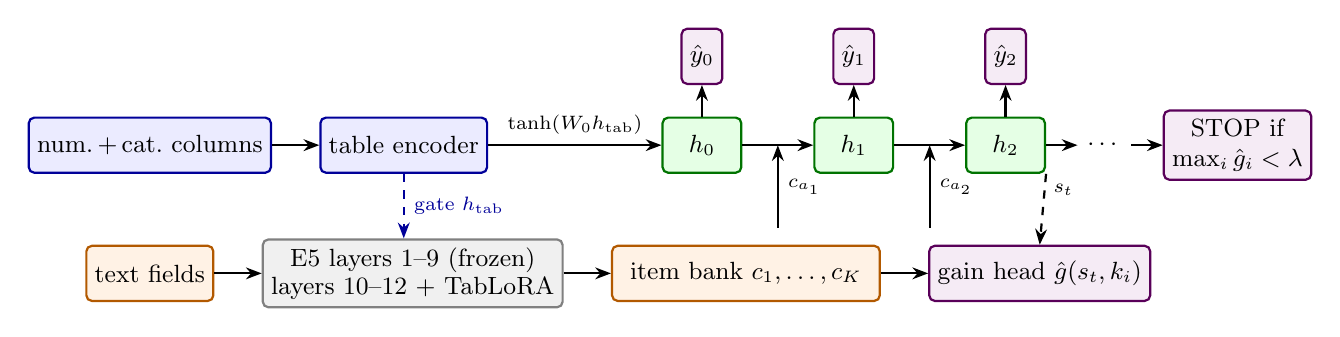
\begin{tikzpicture}[node distance=4mm and 6mm,
  bx/.style={draw, rounded corners=2pt, thick, align=center, minimum height=7mm, inner sep=3pt, font=\small},
  tb/.style={bx, draw=blue!60!black, fill=blue!8},
  tx/.style={bx, draw=orange!70!black, fill=orange!10},
  rn/.style={bx, draw=green!45!black, fill=green!10, minimum width=10mm},
  hd/.style={bx, draw=violet!70!black, fill=violet!8},
  fz/.style={bx, draw=gray, fill=gray!12},
  ar/.style={-{Stealth[length=2mm]}, thick}]
  \node[tb] (row) {num.\,+\,cat.\ columns};
  \node[tb, right=of row] (enc) {table encoder};
  \node[rn, right=22mm of enc] (h0) {$h_0$};
  \node[rn, right=9mm of h0] (h1) {$h_1$};
  \node[rn, right=9mm of h1] (h2) {$h_2$};
  \node[font=\small, right=4mm of h2] (dots) {$\cdots$};
  \node[hd, right=4mm of dots] (stop) {STOP if\\$\max_i \hat g_i<\lambda$};
  \foreach \t in {0,1,2} { \node[hd, above=4mm of h\t] (y\t) {$\hat y_\t$}; \draw[ar] (h\t) -- (y\t); }
  \draw[ar] (row) -- (enc); \draw[ar] (enc) -- node[above, font=\scriptsize]{$\tanh(W_0\htab)$} (h0);
  \draw[ar] (h0) -- (h1); \draw[ar] (h1) -- (h2); \draw[ar] (h2) -- (dots); \draw[ar] (dots) -- (stop);
  \node[tx, below=9mm of row] (txt) {text fields};
  \node[fz, right=of txt] (e5) {E5 layers 1--9 (frozen)\\[-1pt]layers 10--12 + TabLoRA};
  \node[tx, right=6mm of e5, minimum width=34mm] (bank) {item bank $c_1,\dots,c_K$};
  \node[hd, right=6mm of bank] (gain) {gain head $\hat g(s_t,k_i)$};
  \draw[ar] (txt) -- (e5); \draw[ar] (e5) -- (bank); \draw[ar] (bank) -- (gain);
  \draw[ar, dashed, blue!60!black] (enc.south) -- node[right, font=\scriptsize]{gate $\htab$} (e5.north -| enc.south);
  \draw[ar] ($(h0)!0.5!(h1)+(0,-1.05)$) -- node[right, font=\scriptsize]{$c_{a_1}$} ($(h0)!0.5!(h1)$);
  \draw[ar] ($(h1)!0.5!(h2)+(0,-1.05)$) -- node[right, font=\scriptsize]{$c_{a_2}$} ($(h1)!0.5!(h2)$);
  \draw[ar, dashed] (h2.south east) -- node[above right, pos=0.45, font=\scriptsize]{$s_t$} (gain.north);
\end{tikzpicture}}
\caption{The reader: the table initialises a 2-layer GRU and gates the LoRA adapters of E5's top layers; at each step the gain head scores unread items, the reader consumes the best one, and $\hat y_t$ is available after every step.}
\label{fig:arch}
\end{figure}

\textbf{Text items.}
Each text field is split into sentences, merged or cut into chunks of at most 48 words (a field's chunks beyond the eighth merge into one tail item).
Items are allocated round-robin across fields up to $K=\max(8,\#\text{fields})$ per row, so every field has at least one item; the kept items contain every word of the row on 13 of the 20 datasets (Appendix~\ref{app:cov}).
Each item is verbalised as \texttt{passage: <column>: <chunk>} and embedded with E5-small-v2~\cite{wang2022e5} ($e_i\in\mathbb{R}^{384}$); inside the model it becomes
$c_i=\mathrm{LN}(W_{\text{item}}e_i + W_{\text{name}}\,\mathrm{E5}(\text{field name}) + p_{\text{pos}(i)})\in\mathbb{R}^{128}$.

\textbf{Table encoder and anytime reader.}
Each column becomes a token $x_jw_j+m_ju_j+n_j$ (quantile-normalised numerical; $m_j$ marks missingness) or $\mathrm{Emb}(v_j)+n_j$ (categorical), where $n_j$ is a projected E5 embedding of the column name.
An MLP maps the tokens to $\htab\in\mathbb{R}^{128}$, which initialises both layers of a GRU~\cite{cho2014gru}.
After reading items $a_1,\dots,a_t$ the state is $s_t=[h^{(2)}_t;\ \tfrac1t\sum_{\tau\le t}c_{a_\tau};\ \htab]$ (the mean is zero at $t=0$), and an MLP predicts $f(s_t)$.
Training samples a fresh random reading order per batch and averages the loss over all prefixes:
\begin{equation}
\mathcal{L}_{\text{read}}=\tfrac12\cdot\tfrac{1}{n+1}\textstyle\sum_{t=0}^{n}\ell\big(f(s_t),y\big)+\tfrac12\,\ell\big(f(s_n),y\big),
\end{equation}
with $n\le K$ the row's items and $\ell$ cross-entropy (classification) or MSE on the standardised target, so $f$ is valid after \emph{any} subset of reads.

\textbf{Expected-gain policy.}
With the reader frozen, a head $\hat g(s_t,k_i)=\mathrm{MLP}([s_t;k_i])$ regresses the observed gain of reading item $i$ next, $\Delta_i(s_t)=\ell(f(s_t),y)-\ell(f(s_t\oplus c_i),y)$, over all unread items at states visited by an $\varepsilon$-greedy roll-in on held-out rows (DAgger style~\cite{ross2011dagger}).
\emph{Content} keys are $k_i=c_i$; \emph{metadata} keys use only field and position, so unread content is not inspected.
At inference the head needs no label: read $\arg\max_i\hat g$ while $\max_i\hat g\ge\lambda$, with $\lambda$ bisected on validation rows for a target fraction of items.
A pointer network imitating a label-aware greedy oracle was no better than random in pilots, plausibly because the oracle's choices depend on $y$.

\textbf{TabLoRA.}
Joint TAR tunes E5 to the target but encodes a sentence the same way in every row.
We add LoRA adapters ($r=16$, $\alpha=32$) to the query, key, value, attention-output and both feed-forward maps of E5's last three layers (MulTaBench's TAR placement) and gate their rank space with the row's table encoding:
\begin{equation}
W x\ \mapsto\ W x+\tfrac{\alpha}{r}\,B\,\mathrm{diag}\big(1+\tanh(G_W\,\htab)\big)\,A\,x ,
\end{equation}
with $B$ and every $G_W$ initialised at zero, so training starts from frozen E5 and from plain LoRA.
Training has two phases: the reader is fit with frozen items (as above), then the adapters and gates are trained through $\mathcal{L}_{\text{read}}$ with the reader fixed (lr $10^{-3}$, batch 64, at most 10 epochs, patience 3, fp16).
Hidden states entering layer 10 are cached once per item (truncated at 128 tokens), so each step runs only the top three layers.

\textbf{Cross-fitted reader signals and heads.}
For full-budget accuracy we pair the reader with tabular learners on the Joint-Frozen frame (structured columns + PCA-30 of each field's whole-text E5 embedding).
To avoid training-row leakage the reader is \emph{cross-fitted}: three readers are trained on two thirds of the training rows each; every training row is predicted by the reader that did not see it, and test rows get the mean of the three.
TabM and TabPFN-2.5 are fit on the frozen frame alone; for each, a convex weight $w\in\{0,0.05,\dots,1\}$ between learner and read-all reader is tuned on a held-out 20\% of the training rows, on which the reader's predictions are out-of-fold.
The final prediction is the unweighted mean of the two blends; this choice and all hyperparameters were fixed before the five-split evaluation (fold-0 pilots on three datasets informed them).
As in MulTaBench, TabPFN is not used beyond 10 classes (Spotify, Wine), where TabM's blend is used alone.

%======================================================================
\section{Experiments}

\paragraph{Setup.}
We use all 20 MulTaBench text datasets (10 classification: binary or macro one-vs-rest AUROC; 10 regression: $R^2$) under the paper protocol: random holdout splits (seed $42+$fold, test $\le$2{,}000 and train $\le$10{,}000 rows) ported from the official code, five splits per dataset, on pinned dataset revisions.
The reader uses one configuration everywhere ($d=128$, dropout 0.2, AdamW lr $10^{-3}$, 100 epochs, patience 15 on an inner split); TabLoRA's settings were chosen on inner-validation loss of one pilot (Jigsaw, fold 0).
TabM and TabPFN-2.5 run with their default settings (TabM early-stops on the same 20\% split).
Local baselines are run on our exact rows; external references are the official leaderboard scores for the same split seeds (row identity unverified, so no significance test against them).
Following Dem\v{s}ar~\cite{demsar2006statistical}, folds are averaged per dataset and two-sided Wilcoxon signed-rank tests run over datasets, separately for AUROC and $R^2$.
Training used one T4 GPU (TabLoRA: \loraMinutes{} min per dataset split for all three readers).

\begin{table}[t]
\caption{Full-budget accuracy, dataset means (folds averaged per dataset).
W/T/L: datasets where Ours wins, ties or loses against that row; $^{*}$: two-sided Wilcoxon $p<0.05$ (local rows only).
$^{\dagger n}$: available for $n$ datasets only; [ ]: Ours on those $n$.}
\label{tab:main}
\centering
\footnotesize
\begin{tabular}{@{}lcccc@{}}
\toprule
 & \multicolumn{2}{c}{Classification (10, AUROC)} & \multicolumn{2}{c}{Regression (10, $R^2$)} \\
\cmidrule(lr){2-3}\cmidrule(lr){4-5}
Method & mean & Ours W/T/L & mean & Ours W/T/L \\
\midrule
\multicolumn{5}{@{}l}{\emph{Ours (cross-fitted readers, local heads)}} \\
Reader, frozen E5 items & 0.890 & 10/0/0$^{*}$ & 0.651 & 10/0/0$^{*}$ \\
Reader, TabLoRA items & 0.903 & 10/0/0$^{*}$ & 0.672 & 10/0/0$^{*}$ \\
TabM Frozen + TabLoRA reader & 0.910 & 8/2/0$^{*}$ & 0.724 & 9/0/1$^{*}$ \\
TabPFN-2.5 Frozen + TabLoRA reader & 0.897$^{\dagger8}$\,[0.898] & 4/0/4 & 0.734 & 4/0/6 \\
\textbf{Ours}: mean of the two blends & 0.913 &  & 0.738 &  \\
\midrule
\multicolumn{5}{@{}l}{\emph{Local baselines (identical rows)}} \\
v1 Blend: CatBoost Frozen + reader & 0.900 & 9/0/1$^{*}$ & 0.702 & 10/0/0$^{*}$ \\
CatBoost, Joint Frozen & 0.887 & 10/0/0$^{*}$ & 0.684 & 10/0/0$^{*}$ \\
TabM, Joint Frozen & 0.895 & 10/0/0$^{*}$ & 0.716 & 10/0/0$^{*}$ \\
TabPFN-2.5, Joint Frozen & 0.884$^{\dagger8}$\,[0.898] & 6/0/2 & 0.729 & 5/0/5 \\
\midrule
\multicolumn{5}{@{}l}{\emph{MulTaBench reference, Joint TAR (LoRA-tuned E5)}} \\
CatBoost, Joint TAR & 0.907 & 9/0/1 & 0.716 & 9/0/1 \\
LightGBM, Joint TAR & 0.894 & 9/0/1 & 0.702 & 10/0/0 \\
TabM, Joint TAR & 0.911 & 5/0/5 & 0.728 & 9/0/1 \\
TabPFN-2.5, Joint TAR & 0.900$^{\dagger8}$\,[0.898] & 3/0/5 & 0.732 & 4/0/6 \\
\bottomrule
\end{tabular}

\end{table}

\paragraph{Full-budget accuracy (Table~\ref{tab:main}).}
Our model improves on every local baseline on both task families: on our previous CatBoost blend by \oursVsVoneClsDelta{} AUROC (\oursVsVoneClsWins/\oursVsVoneClsN{} datasets, $p=\oursVsVoneClsP$) and \oursVsVoneRegDelta{} $R^2$ (\oursVsVoneRegWins/\oursVsVoneRegN, $p=\oursVsVoneRegP$), and on Joint-Frozen TabM by \oursVsTabMClsDelta{} AUROC ($p=\oursVsTabMClsP$) and \oursVsTabMRegDelta{} $R^2$ ($p=\oursVsTabMRegP$).
Against the Joint TAR references, which fine-tune E5 on the target, it is level with TabM TAR on classification (\oursVsLbTabMTarClsDelta, \oursVsLbTabMTarClsWins/\oursVsLbTabMTarClsN{} wins) and ahead on regression (\oursVsLbTabMTarRegDelta, \oursVsLbTabMTarRegWins/\oursVsLbTabMTarRegN), and \oursVsLbBestTarClsDelta{} AUROC and \oursVsLbBestTarRegDelta{} $R^2$ from the per-dataset best of the four TAR learners (Appendix~\ref{app:per}).

\begin{table}[t]
\caption{Where the gains come from: dataset-level mean difference, wins and Wilcoxon $p$ (all five folds unless noted).}
\label{tab:abl}
\centering
\footnotesize
\setlength{\tabcolsep}{4pt}
\begin{tabular}{@{}lcccccc@{}}
\toprule
 & \multicolumn{3}{c}{Classification (AUROC)} & \multicolumn{3}{c}{Regression ($R^2$)} \\
\cmidrule(lr){2-4}\cmidrule(lr){5-7}
Comparison (left $-$ right) & $\Delta$ & wins & $p$ & $\Delta$ & wins & $p$ \\
\midrule
TabLoRA vs.\ frozen-E5 items, reader alone & +0.011 & 9/10 & 0.004 & +0.034 & 3/3 & -- \\
TabLoRA vs.\ frozen-E5 items, final system & +0.006 & 9/10 & 0.064 & +0.001 & 1/3 & -- \\
Table gate vs.\ plain LoRA, reader (fold 0) & -- & -- & -- & -- & -- & -- \\
Adding the reader to TabM Frozen & +0.012 & 9/10 & 0.037 & +0.007 & 3/3 & -- \\
Adding the reader to TabPFN-2.5 Frozen & +0.013 & 5/8 & 0.094 & +0.001 & 2/3 & -- \\
Blend vs.\ stacking (TabM) & 0.000 & 3/10 & 0.432 & +0.001 & 1/3 & -- \\
Two heads vs.\ TabM only & +0.003 & 7/10 & 0.016 & +0.018 & 3/3 & -- \\
\bottomrule
\end{tabular}

\end{table}

\paragraph{Ablations (Table~\ref{tab:abl}).}
TabLoRA makes the reader itself better (\loraReaderClsDelta{} AUROC, \loraReaderClsWins/\loraReaderClsN{} datasets; \loraReaderRegDelta{} $R^2$, \loraReaderRegWins/\loraReaderRegN), largest where the text carries the signal (Jigsaw \sJigsawToxicityR{}$\to$\sJigsawToxicityRLora{} AUROC).
After blending with the learners, part of this gain is absorbed (\loraSystemClsDelta{} and \loraSystemRegDelta), because the learners already see the frozen text embeddings.
The reader adds to both learners, and the two blends are better than either alone: their errors differ.
Blending and stacking the reader's predictions as features into TabM perform alike, so we keep the simpler blend.

\begin{table}[t]
\caption{Selective reading (frozen-item reader): gain policy minus a random reader with the same per-row number of reads, per nominal budget. ``read'': achieved test fraction; $p_{\text{Holm}}$: Wilcoxon $p$, Holm-adjusted~\cite{holm1979} over the 8 key$\times$budget cells per family.}
\label{tab:budget}
\centering
\footnotesize
\setlength{\tabcolsep}{4pt}
\begin{tabular}{@{}llcccccccc@{}}
\toprule
 & & \multicolumn{4}{c}{Classification ($\Delta$AUROC)} & \multicolumn{4}{c}{Regression ($\Delta R^2$)} \\
\cmidrule(lr){3-6}\cmidrule(lr){7-10}
Keys & Budget & read & $\Delta$ & W/T/L & $p_{\text{Holm}}$ & read & $\Delta$ & W/T/L & $p_{\text{Holm}}$ \\
\midrule
content & 10\% & 10\% & +0.026 & 9/1/0 & 0.031 & 10\% & +0.051 & 10/0/0 & 0.016 \\
content & 25\% & 25\% & +0.024 & 9/1/0 & 0.031 & 25\% & +0.053 & 10/0/0 & 0.016 \\
content & 50\% & 50\% & +0.014 & 9/1/0 & 0.031 & 50\% & +0.039 & 10/0/0 & 0.016 \\
content & 75\% & 75\% & +0.007 & 9/1/0 & 0.031 & 75\% & +0.023 & 9/0/1 & 0.018 \\
\midrule
metadata & 10\% & 9\% & +0.010 & 8/1/1 & 0.031 & 10\% & +0.037 & 10/0/0 & 0.016 \\
metadata & 25\% & 25\% & +0.018 & 8/1/1 & 0.031 & 25\% & +0.039 & 9/0/1 & 0.018 \\
metadata & 50\% & 54\% & +0.012 & 8/1/1 & 0.031 & 50\% & +0.034 & 9/0/1 & 0.018 \\
metadata & 75\% & 76\% & +0.007 & 9/1/0 & 0.031 & 75\% & +0.021 & 9/0/1 & 0.016 \\
\bottomrule
\end{tabular}

\end{table}

\paragraph{Selective reading (Table~\ref{tab:budget}).}
These experiments use the reader with frozen items.
At 10\% of the items the content policy beats the matched random reader by \gainContentTenClsDelta{} AUROC (\gainContentTenClsWins/10 datasets) and \gainContentTenRegDelta{} $R^2$ (\gainContentTenRegWins/10); all 16 key$\times$budget comparisons are significant after Holm correction, and metadata keys, which never see unread content, also win at every budget.
Against random items with the same \emph{total} reads spread over rows (Appendix~\ref{app:ctl}), the 10\% gap widens to \ctlTotalContentTenClsDelta{} AUROC: choosing \emph{which rows} to read matters as much as which items.
At 10\% of the items the policy recovers a median \recContentTen{} of what reading everything adds over the table alone (random: \recRandomContentTen).

%======================================================================
\section{Conclusion}

Conditioning text reading on the table helps at both levels we tried: what to read (a label-free gain policy beats budget-matched random reading at every budget) and how to read it (TabLoRA improves the reader).
Cross-fitted and blended with Joint-Frozen TabM and TabPFN-2.5, the reader significantly improves on all local baselines and reaches the Joint TAR references without fine-tuning E5 on the learners' side.
\textbf{Limitations:} TabLoRA's gain shrinks once strong learners are added; the selective-reading results use the frozen-item reader; all items are embedded before selection, so the read fraction is not a compute saving; the $K$-item cap drops long text (Zomato); TabPFN needs its training rows at inference.
\textbf{Future work:} TAR-tuned frozen frames for the learners, lazy encoding of selected items only, and a multi-step gain policy.

\bibliographystyle{plain}
\bibliography{references}

\appendix
\makeatletter\setlength{\@fptop}{0pt}\setlength{\@fpsep}{12pt plus 1fil}\makeatother % top-align appendix float pages
\section{Per-dataset results}\label{app:per}
\begin{table}[h]
\caption{Fold-mean scores per dataset. v1: CatBoost Frozen + frozen-item reader blend; TabM, PFN: Joint-Frozen learners on our rows; R / R$_{\text{LoRA}}$: cross-fitted reader with frozen / TabLoRA items; Ours $\pm$ fold std. LB: MulTaBench leaderboard (TabM TAR and the best of four TAR learners) for matching split seeds. Bold: best of our columns.}
\centering
\scriptsize
\setlength{\tabcolsep}{3pt}
\resizebox{\linewidth}{!}{\begin{tabular}{@{}lcccccccc@{}}
\toprule
 & \multicolumn{6}{c}{Ours and local baselines (identical rows)} & \multicolumn{2}{c}{LB Joint TAR} \\
\cmidrule(lr){2-7}\cmidrule(lr){8-9}
Dataset & v1 & TabM & PFN & R & R$_{\text{LoRA}}$ & Ours & TabM & best \\
\midrule
\multicolumn{9}{@{}l}{\emph{Classification (AUROC)}} \\
Fake Job Posting & 0.912 & 0.948 & 0.952 & 0.918 & 0.922 & \textbf{0.961} & 0.934 & 0.934 \\
Jigsaw Toxicity & 0.841 & 0.805 & 0.805 & 0.843 & \textbf{0.898} & \textbf{0.898} & 0.917 & 0.927 \\
Kickstarter & 0.741 & 0.745 & 0.743 & 0.732 & 0.740 & \textbf{0.752} & 0.760 & 0.760 \\
DS Salary & 0.825 & 0.829 & 0.833 & 0.823 & 0.829 & \textbf{0.835} & 0.832 & 0.834 \\
Michelin & 0.913 & 0.914 & 0.913 & 0.903 & 0.909 & \textbf{0.918} & 0.919 & 0.926 \\
Product Sentiment & 0.901 & 0.907 & \textbf{0.912} & 0.901 & 0.900 & 0.907 & 0.909 & 0.916 \\
Spotify Genres & \textbf{0.968} & 0.957 & -- & 0.953 & 0.958 & 0.966 & 0.964 & 0.965 \\
US Accidents & 0.972 & 0.970 & \textbf{0.979} & 0.937 & 0.956 & 0.977 & 0.980 & 0.985 \\
Wine Review & 0.978 & 0.976 & -- & 0.976 & 0.980 & \textbf{0.980} & 0.981 & 0.981 \\
Women Clothing & 0.907 & 0.910 & 0.911 & 0.903 & 0.905 & \textbf{0.911} & 0.914 & 0.914 \\
\midrule
\multicolumn{9}{@{}l}{\emph{Regression ($R^2$)}} \\
Babies Prices & 0.890 & 0.880 & \textbf{0.919} & 0.841 & 0.859 & 0.910 & 0.923 & 0.930 \\
Book Price & 0.554 & 0.571 & \textbf{0.616} & 0.434 & 0.491 & 0.602 & 0.555 & 0.579 \\
Book Readability & 0.801 & 0.795 & 0.802 & 0.773 & 0.801 & \textbf{0.809} & 0.800 & 0.836 \\
\bottomrule
\end{tabular}
}
\end{table}

\clearpage
\section{Text coverage of the item representation}\label{app:cov}
\begin{table}[!ht]
\caption{Fold-0 test rows. Items/row: items kept after the cap $K$; rows over $K$: rows with more candidate chunks than $K$; words kept: share of the row's words inside kept items (an upper bound on what E5 sees).}
\centering
\scriptsize
\begin{tabular}{@{}lcccccc@{}}
\toprule
Dataset & text fields & $K$ & words/row & items/row & rows over $K$ & words kept \\
\midrule
\multicolumn{7}{@{}l}{\emph{Classification}} \\
Fake Job Posting & 3 & 8 & 176 & 5.4 & 15\% & 89\% \\
Jigsaw Toxicity & 1 & 8 & 52 & 1.8 & 0\% & 100\% \\
Kickstarter & 3 & 8 & 26 & 3.0 & 0\% & 100\% \\
DS Salary & 5 & 8 & 29 & 4.8 & 0\% & 100\% \\
Michelin & 6 & 8 & 110 & 7.4 & 17\% & 94\% \\
Product Sentiment & 1 & 8 & 18 & 1.0 & 0\% & 100\% \\
Spotify Genres & 3 & 8 & 9 & 3.0 & 0\% & 100\% \\
US Accidents & 6 & 8 & 19 & 6.0 & 0\% & 100\% \\
Wine Review & 2 & 8 & 41 & 2.2 & 0\% & 100\% \\
Women Clothing & 2 & 8 & 62 & 2.7 & 0\% & 100\% \\
\midrule
\multicolumn{7}{@{}l}{\emph{Regression}} \\
Babies Prices & 4 & 8 & 12 & 2.7 & 0\% & 100\% \\
Book Price & 5 & 8 & 176 & 7.4 & 43\% & 77\% \\
Book Readability & 6 & 8 & 185 & 7.8 & 49\% & 90\% \\
Mercari & 6 & 8 & 37 & 5.8 & 1\% & 99\% \\
Montgomery Sal. & 3 & 8 & 9 & 3.0 & 0\% & 100\% \\
Rotten Tomatoes & 13 & 13 & 71 & 12.8 & 1\% & 100\% \\
SCImago Impact & 10 & 10 & 28 & 10.0 & 0\% & 100\% \\
Vancouver Sal. & 2 & 8 & 5 & 2.0 & 0\% & 100\% \\
Video Games & 2 & 8 & 6 & 2.0 & 0\% & 100\% \\
Zomato & 7 & 8 & 1909 & 7.8 & 79\% & 6\% \\
\bottomrule
\end{tabular}

\end{table}

\IfFileExists{generated/tab_controls.tex}{%
\section{Reading controls}\label{app:ctl}
\begin{table}[!ht]
\caption{Frozen-item reader, dataset-level mean difference (wins/datasets) at nominal budgets 10\% and 50\%, all five folds.
\emph{Same total reads}: random items, with the policy's total number of reads spread over rows in proportion to their item counts.
\emph{Same per-row reads}: random items with the policy's per-row counts (as in Table~\ref{tab:budget}).
\emph{Row allocation}: the second random reader minus the first.
\emph{Natural order}: fields and chunks in their stored order, same counts as the first reader.
$^{*}$: Holm-adjusted Wilcoxon $p<0.05$ over the eight key$\times$budget cells.}
\centering
\scriptsize
\setlength{\tabcolsep}{3pt}
\begin{tabular}{@{}llcccc@{}}
\toprule
 & & \multicolumn{2}{c}{Classification ($\Delta$AUROC)} & \multicolumn{2}{c}{Regression ($\Delta R^2$)} \\
\cmidrule(lr){3-4}\cmidrule(lr){5-6}
Comparison & Keys & 10\% & 50\% & 10\% & 50\% \\
\midrule
gain $-$ random (same total reads) & content & +0.053 (10/10)$^{*}$ & +0.019 (10/10)$^{*}$ & +0.122 (10/10)$^{*}$ & +0.068 (10/10)$^{*}$ \\
 & metadata & +0.020 (8/10) & +0.015 (8/10) & +0.086 (10/10)$^{*}$ & +0.060 (10/10)$^{*}$ \\
\midrule
gain $-$ random (same per-row reads) & content & +0.027 (9/10)$^{*}$ & +0.014 (9/10)$^{*}$ & +0.051 (10/10)$^{*}$ & +0.042 (10/10)$^{*}$ \\
 & metadata & +0.014 (9/10)$^{*}$ & +0.013 (8/10)$^{*}$ & +0.038 (10/10)$^{*}$ & +0.038 (10/10)$^{*}$ \\
\midrule
policy row allocation $-$ uniform & content & +0.027 (10/10)$^{*}$ & +0.006 (7/10) & +0.071 (10/10)$^{*}$ & +0.027 (7/10) \\
 & metadata & +0.005 (8/10) & +0.003 (4/10) & +0.048 (10/10)$^{*}$ & +0.022 (7/10) \\
\midrule
gain $-$ natural field order & content & +0.044 (10/10)$^{*}$ & +0.007 (7/10) & +0.123 (10/10)$^{*}$ & +0.086 (10/10)$^{*}$ \\
 & metadata & +0.009 (6/10) & +0.003 (4/10) & +0.088 (10/10)$^{*}$ & +0.079 (8/10) \\
\bottomrule
\end{tabular}

\end{table}
\IfFileExists{generated/tab_fieldmeta.tex}{%
\begin{table}[!ht]
\caption{Adding each text field's presence flag and log word count to the table encoder (fold 0, matched datasets).
Gain $-$ random is the advantage over the per-row matched random reader. $^{*}$: Wilcoxon $p<0.05$.}
\centering
\scriptsize
\begin{tabular}{@{}lcccccc@{}}
\toprule
 & \multicolumn{3}{c}{Classification (AUROC)} & \multicolumn{3}{c}{Regression ($R^2$)} \\
\cmidrule(lr){2-4}\cmidrule(lr){5-7}
 & without & with & $\Delta$ (W/$n$) & without & with & $\Delta$ (W/$n$) \\
\midrule
Reader, table only & 0.753 & 0.778 & +0.025 (9/10)$^{*}$ & 0.430 & 0.467 & +0.037 (8/10)$^{*}$ \\
Reader, read all & 0.889 & 0.887 & $-$0.002 (3/10) & 0.671 & 0.645 & $-$0.026 (2/10) \\
gain $-$ random, content @10\% & +0.028 & +0.017 & $-$0.011 (1/10)$^{*}$ & +0.051 & +0.064 & +0.013 (8/10) \\
gain $-$ random, content @25\% & +0.023 & +0.017 & $-$0.006 (1/10)$^{*}$ & +0.054 & +0.065 & +0.010 (4/10) \\
gain $-$ random, metadata @10\% & +0.016 & +0.009 & $-$0.007 (1/10)$^{*}$ & +0.034 & +0.028 & $-$0.006 (5/10) \\
gain $-$ random, metadata @25\% & +0.018 & +0.015 & $-$0.002 (3/10) & +0.040 & +0.023 & $-$0.017 (2/10)$^{*}$ \\
\bottomrule
\end{tabular}

\end{table}}{}}{}

\end{document}
